\documentclass[aspectratio=169, 10pt]{beamer}

% Packages
\usepackage[utf8]{inputenc}
\usepackage[T1]{fontenc}
\usepackage[french]{babel}
\usepackage{graphicx}
\usepackage{booktabs}
\usepackage{multicol}
\usepackage{caption}
\usepackage{subcaption}

% ---------------------------------------------------
% THÈME ET COULEURS SCIKIT-LEARN
% ---------------------------------------------------
\usetheme{Boadilla}

% Couleurs extraites du logo Scikit-Learn
\definecolor{sklblue}{HTML}{37ABE1}    % Bleu clair Scikit
\definecolor{sklorange}{HTML}{F59D31}  % Orange Scikit
\definecolor{skldarkblue}{HTML}{216093} % Bleu foncé pour contrastes
\definecolor{colortt}{HTML}{0b8509}  % Vert clair pour le code

% Application des couleurs au thème Beamer
\setbeamercolor{structure}{fg=sklblue}
\setbeamercolor{palette primary}{bg=sklblue, fg=black}
\setbeamercolor{palette secondary}{bg=skldarkblue, fg=white}
\setbeamercolor{palette tertiary}{bg=sklorange, fg=white}
\setbeamercolor{title}{bg=sklblue, fg=black}
\setbeamercolor{frametitle}{bg=sklblue, fg=black}
\setbeamercolor{item}{fg=sklorange}
\setbeamercolor{alerted text}{fg=sklorange}

% Suppression des symboles de navigation en bas
\setbeamertemplate{navigation symbols}{}


% ---------------------------------------------------
% MES COMMANDES
% ---------------------------------------------------
\newcommand{\mytexttt}[1]{\texttt{\textbf{\textcolor{colortt}{#1}}}}
\newcommand{\bhref}[2]{\textcolor{blue}{\href{#1}{#2}}}

% ---------------------------------------------------
% MÉTADONNÉES
% ---------------------------------------------------
\title[Prédiction de revenus - Adult Dataset]{Projet Machine Learning / Maths pour l'apprentissage}
\subtitle{Adult Dataset : de l'expérimentation à la professionnalisation}
\author{Matthieu PELINGRE}
\institute[M2 SDD]{Master 2 SDD}
\date{11 avril 2026}

\begin{document}

% --- SLIDE 1 : TITRE ---
\begin{frame}
    \titlepage
\end{frame}

% --- SLIDE 2 : LE DÉFI & LE FIL ROUGE ---
\begin{frame}{Contexte : un défi personnel}
    \textbf{L'objectif :} Prédire si un individu gagne \textbf{> 50 000 \$} par an à partir de données censitaires.
    
    \pause
    \vspace{0.5cm}
    \textbf{Pourquoi ce dataset ?} \pause ~$\rightarrow$ confrontation directe avec mon "Moi" d'il y a quelques années : \pause
    \begin{itemize}
        \item \textbf{À l'époque :} Découverte des librairies Scikit-Learn et XGBoost. Approche naïve, \textit{Data Leakage} et déséquilibre ignoré, peu de sélection des variables, pas d'optimisation.
        \pause
        \item \textbf{Aujourd'hui :} Démarche plus rigoureuse, création d'un \mytexttt{Pipeline} robuste, lutte contre le déséquilibre des classes et assurer l'explicabilité.
    \end{itemize}

\pause
    \vspace{0.5cm}
    \begin{alertblock}{Problématique}
        Classe minoritaire à \textbf{24,2 \%}. \\ Objectif : maximiser le \textbf{F1-Score (macro)} pour garantir un équilibre Précision/Rappel.
    \end{alertblock}
\end{frame}


% --- SLIDE 3 : ANALYSE EXPLORATOIRE (EDA) ---
\begin{frame}{Analyse Exploratoire des Données (EDA)}
    \textbf{Que révèlent les données ?} \pause
    \begin{itemize}
        \item<2-> Les hauts revenus sont corrélés à l'\textbf{âge} (maturité professionnelle), au \textbf{niveau d'éducation} et à des \textbf{gains financiers atypiques} (\mytexttt{capital-gain}).
        \item<3-> Le \textbf{statut marital} (\textit{Married-civ-spouse}) est le discriminant catégoriel absolu (idem pour \mytexttt{relationship} $\rightarrow$ redondance).
    \end{itemize}
    
\vspace{0.3cm}
\begin{figure}[]
    \centering
    \visible<2->{
    \begin{subfigure}[t]{0.45\textwidth}
        \centering
        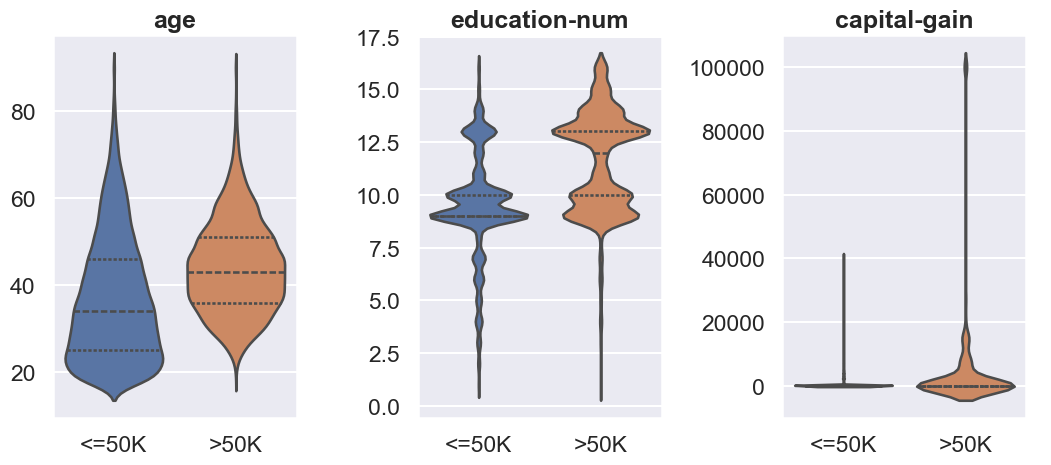
\includegraphics[width=\linewidth]{pictures/EDA/var_num.png}
        \caption{Distributions par classe de revenu.}
    \end{subfigure}
    }
    \hfill
    \visible<3->{
    \begin{subfigure}[t]{0.50\textwidth}
        \centering
        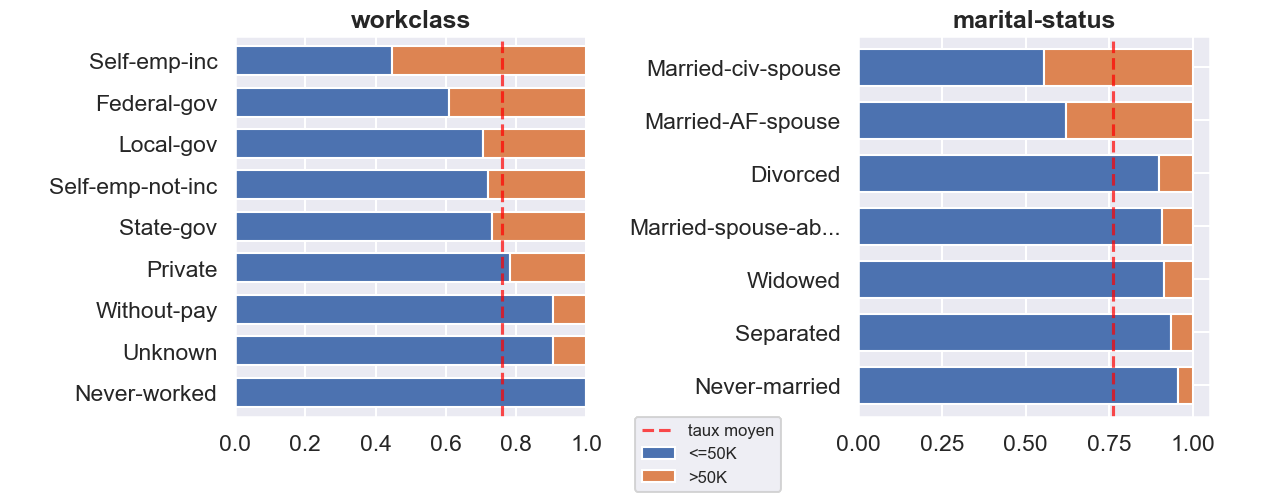
\includegraphics[width=\linewidth]{pictures/EDA/var_cat.png}
		\caption{Taux de >50K par modalité.}
    \end{subfigure}
    }
\end{figure}
\end{frame}

% --- SLIDE 4 : SÉLECTION DES FEATURES ---
\begin{frame}{Sélection des caractéristiques (Feature Selection)}
    \textbf{Élaguer pour réduire le bruit}
    
    À mes débuts, j'avais conservé presque toutes les variables. L'analyse statistique a changé la donne :
    
    \vspace{0.3cm}
    \begin{itemize}
        \item<2-> \textbf{Confirmation statistiques :} Calcul du V de Cramér et de l'Information Mutuelle (MI).
        \item<3-> \textbf{Gestion de la redondance :} \mytexttt{relationship} écartée au profit de \mytexttt{sex} et \mytexttt{marital-status}.
        \item<4-> \textbf{Suppression du bruit :} \mytexttt{race} et \mytexttt{native-subregion} exclues car pouvoir prédictif quasi nul.
    \end{itemize}
    
\vspace{0.1cm}
\begin{figure}[]
    \centering
    \visible<3->{
    \begin{subfigure}[t]{0.30\textwidth}
        \centering
        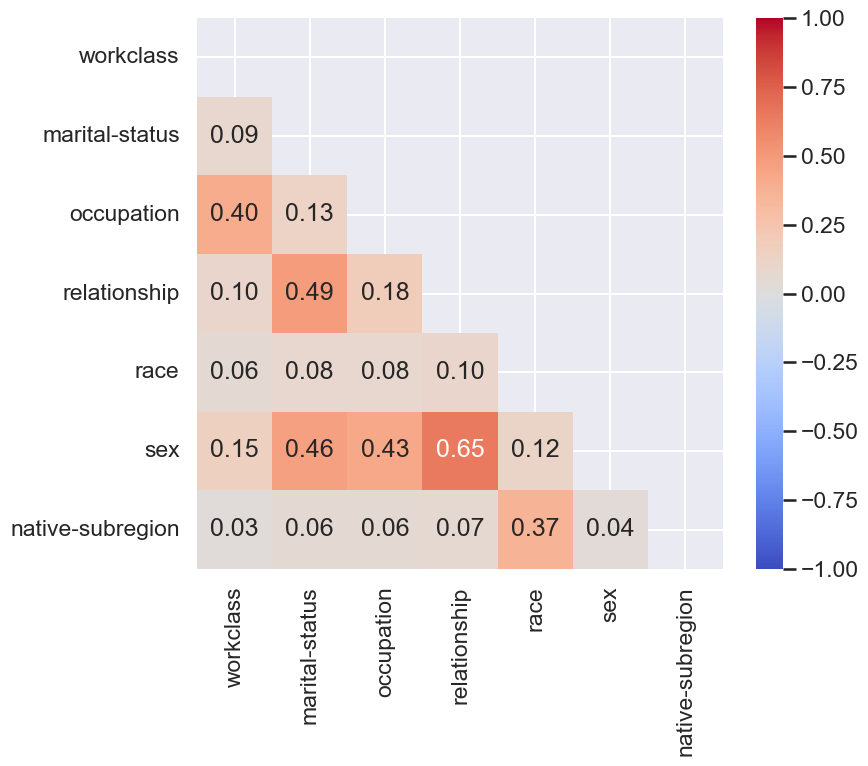
\includegraphics[width=\linewidth]{pictures/selection/corr_cramer.png}
        \caption{V de Cramér}
    \end{subfigure}
    }
    \hspace{1.5cm}
    \visible<4->{
    \begin{subfigure}[t]{0.35\textwidth}
        \centering
        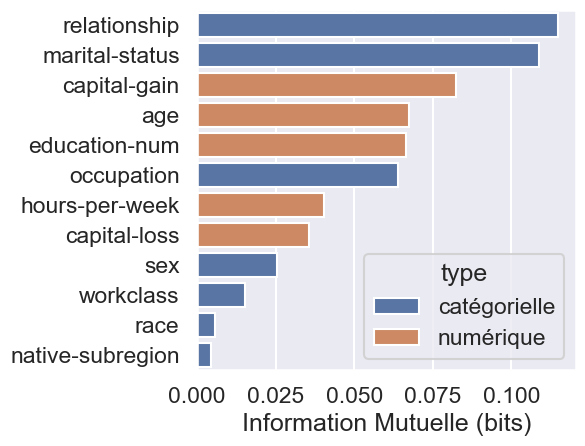
\includegraphics[width=\linewidth]{pictures/selection/mutual_info.png}
		\caption{Information Mutuelle (MI).}
    \end{subfigure}
    }
\end{figure}

\end{frame}


% --- SLIDE 5 : LE PIÈGE DE LA PRÉPARATION ---
\begin{frame}{Préparation des données : évolution de la méthode}

\textbf{Dans les deux cas} : suppression de \mytexttt{fnlwgt} (poids stat de pondération) et de \mytexttt{education}, redondante avec \mytexttt{education-num} plus intéressante (encodage selon échelle ordinale).
\pause

\vspace{0.3cm}
    \begin{columns}[T]
        \begin{column}{0.48\textwidth}
            \textbf{Les erreurs formatrices (2021) :}
            \begin{itemize}
                \item<3-> Split aléatoire sans seed (non reproductibles).
                \item<4-> \mytexttt{pd.get\_dummies} appliqué \textit{avant} séparation $\rightarrow$ \alert{\textbf{Data Leakage}}.
                \item<5-> \textbf{Valeurs manquantes :} Ignorées silencieusement (supprimées de fait lors de l'encodage naïf).
            \end{itemize}
        \end{column}
        
        \begin{column}{0.48\textwidth}
            \textbf{La robustesse (2026) :}
            \begin{itemize}
                \item<3-> Split fixé (\mytexttt{random\_state=42}).
                \item<4-> \textbf{Encapsulation} dans des \mytexttt{Pipeline} Scikit-Learn (zéro fuite), facilité d'usage.
                %\item \textbf{Encapsulation} dans des \mytexttt{Pipeline} Scikit-Learn : zéro fuite (le \mytexttt{StandardScaler} et le \mytexttt{OneHotEncoder} n'apprennent \textit{que} sur le \mytexttt{train}), facilité d'usage / mise en prod.
                \item<5-> \textbf{Traitement ciblé des NaN :}
                \begin{itemize}
                    \item<6->[\textcolor{sklorange}{$\rightarrow$}] \textit{MCAR} : Lignes exclues.
                    \item<7->[\textcolor{sklorange}{$\rightarrow$}] \textit{MNAR} : Remplacées par la modalité \textit{Unknown} (vectrice d'information).
                \end{itemize}
            \end{itemize}
        \end{column}
    \end{columns}
\end{frame}






% --- SLIDE 6 : MODÉLISATION & OPTIMISATION ---
\begin{frame}{Modélisation et optimisation}

    \begin{alertblock}{Interfaçage différent en 2021}
À l'époque, j'avais utilisé l'API standard (plus optimisée sur GPU) et fait uniquement une \textbf{3-fold CV}. Maintenant, puissance de calcul moins problématique, utilisation de l'API Scikit-Learn avec l'objet \mytexttt{XGBClassifier}.
    \end{alertblock}
    \vspace{0.3cm}
    
    \pause
    \textbf{Les modèles testés :} Random Forest (parallèle) et XGBoost (séquentiel), modèles ensemblistes très performants sur données tabulaires.
    
    \pause
    \vspace{0.1cm}
    \textbf{Stratégie d'optimisation (\mytexttt{RandomizedSearchCV}) :}
    \begin{itemize}
        \item Maximisation du F1-Score (macro).
    \pause
        \item \textbf{Surprise sur le déséquilibre :} L'algorithme a rejeté les poids de compensation (\mytexttt{scale\_pos\_weight}, \mytexttt{class\_weight}).
    \pause
        \item \textbf{Adaptation structurelle :} XGBoost a compensé la rareté en favorisant de nombreux arbres trapus (faible \mytexttt{max\_depth}) avec un apprentissage lent (\mytexttt{learning\_rate = 0.04}). Random Forest lui a utilisé des arbres profonds (\mytexttt{max\_depth=20}) mais élagués (\mytexttt{min\_samples\_leaf=4}).
    \end{itemize}
\end{frame}

% --- SLIDE 7 : BAGGING vs BOOSTING (RÉSULTATS) ---
\begin{frame}{Résultats finaux (1/2) : bagging vs boosting}

    \begin{table}[]
        \centering
        \begin{tabular}{lccccc}
        \toprule
\textbf{Modèle} & \textbf{Acc} & \textbf{P} & \textbf{R} & \textbf{F1-macro} & \textbf{AUC-ROC} \\
		\midrule
DummyClassifier          & \alert{\textbf{0.753}} & \textcolor{gray}{0.376} & \textcolor{gray}{0.500} & \textcolor{gray}{\textbf{0.429}} & \textcolor{gray}{\textbf{0.500}} \\
Random Forest            & 0.862 & 0.833 & 0.775 & 0.798 & 0.920 \\
\textbf{XGBoost}         & \textbf{0.871} & \alert{\textbf{0.843}} & \textbf{0.794} & \textbf{0.814} & \textbf{0.932} \\
        \bottomrule
        \end{tabular}
    \end{table}

    \vspace{0.5cm}
    \pause
\textbf{Méthodologie effcace :}
\begin{itemize}
    \pause
    \item Random Forest surpasse largement sa \bhref{https://archive.ics.uci.edu/dataset/2/adult}{baseline} ($Acc_{max} =$ 0.858 et $P_{max} =$ 0.811).
    \pause
    \item \textbf{XGBoost} devance Random Forest. 
    \pause
    \item \textbf{XGBoost} dépasse de peu la Précision sa \bhref{https://archive.ics.uci.edu/dataset/2/adult}{baseline} ($Acc_{max} =$ 0.877 et $P_{max} =$ \alert{\textbf{0.842}}).
    \pause
    \item Capacité de discrimination validée par AUC-ROC.
\end{itemize}
\end{frame}


% --- SLIDE 7b : LE SAUT QUALITATIF (RÉSULTATS) ---
\begin{frame}{Résultats finaux (2/2) : le saut qualitatif}
    \begin{table}[]
        \centering
        \begin{tabular}{lcccc}
        \toprule
        \textbf{Modèle XGBoost} & \textbf{Acc} & \textbf{P} & \textbf{R} & \textbf{F1-Score} \\
        \midrule
        \textcolor{gray}{\textit{DummyClassifier}} & \alert{\textbf{0.753}} & \textcolor{gray}{0.376} & \textcolor{gray}{\textbf{0.500}} & \textcolor{gray}{0.429} \\
        \midrule
        Première approche (2021) & \textcolor{gray}{0.869} & \textcolor{gray}{0.784} & \alert{\textbf{0.609}} & \textcolor{gray}{\textbf{0.686}} \\
        \textbf{Version M2 SDD (2026)} & \textbf{0.871} & \textbf{0.843} & \alert{\textbf{0.794}} & \textbf{0.814} \\
        \bottomrule
        \end{tabular}
    \end{table}
    \pause

    \vspace{0.5cm}
    \pause
    \textbf{Pourquoi des gens utilisent encore l'Accuracy ?}\\
    
    \pause
    Exactitude (Accuracy) quasi identique (+0.2 \%), mais l'approche \textit{"moderne"} a permis de bondir de \textbf{+18.5 points sur le Rappel}.
    \pause
    
    Le modèle ne rate plus la classe minoritaire !
\end{frame}


% --- SLIDE 8 : INTERPRÉTABILITÉ (GLOBAL) ---
\begin{frame}{Interprétabilité globale : que comprend le modèle ?}
    \textbf{Variables prédictives dominantes} (Feature Importance XGBoost) :
    \vspace{0.1cm}
    \begin{itemize}
        \item<2-> \textbf{45 \% de la décision} repose sur le statut marital.
        \item<3-> Les investissements financiers (\mytexttt{capital-gain}) sont dans le Top 3 (intuitions de l'EDA).
    \end{itemize}
    
    \vspace{0.1cm}
\begin{figure}[]
    \centering
    \visible<2->{
    \begin{subfigure}[t]{0.40\textwidth}
        \centering
        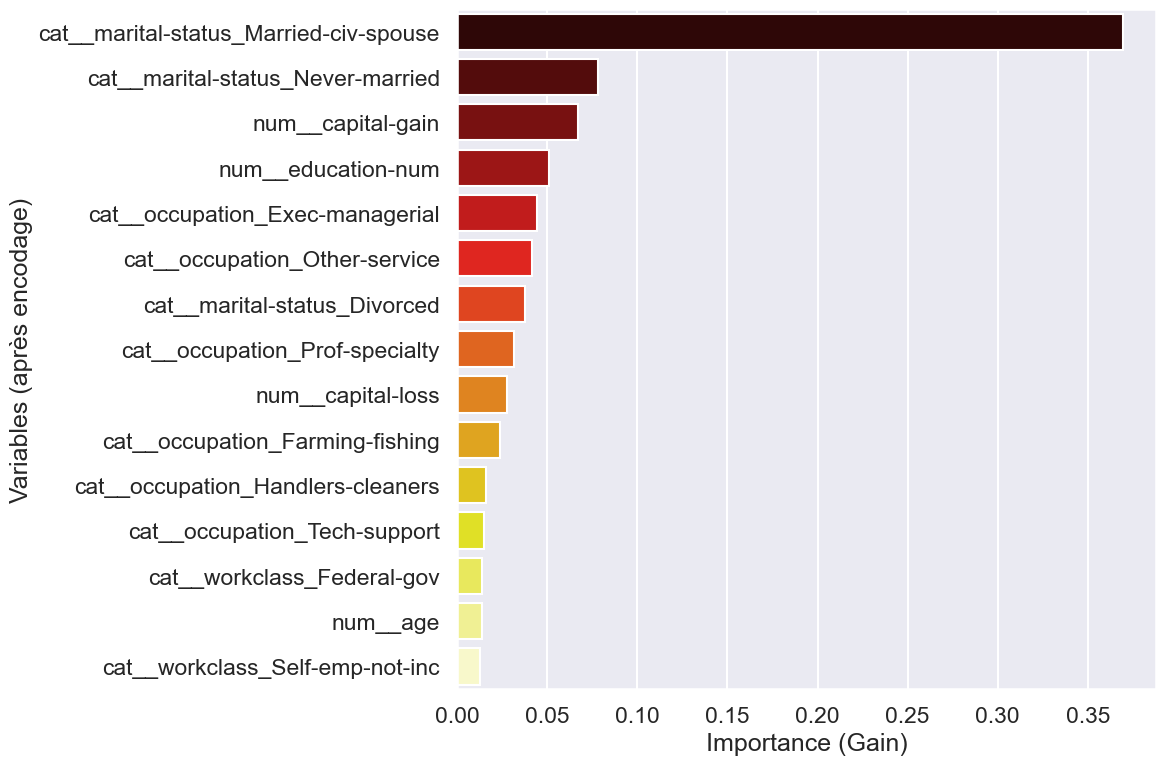
\includegraphics[width=\linewidth]{pictures/importance/feature_importance.png}
        \caption{Importance dans la prédiction (Gain).}
    \end{subfigure}
    }
    \hspace{1.5cm}
    \visible<4->{
    \begin{subfigure}[t]{0.40\textwidth}
        \centering
        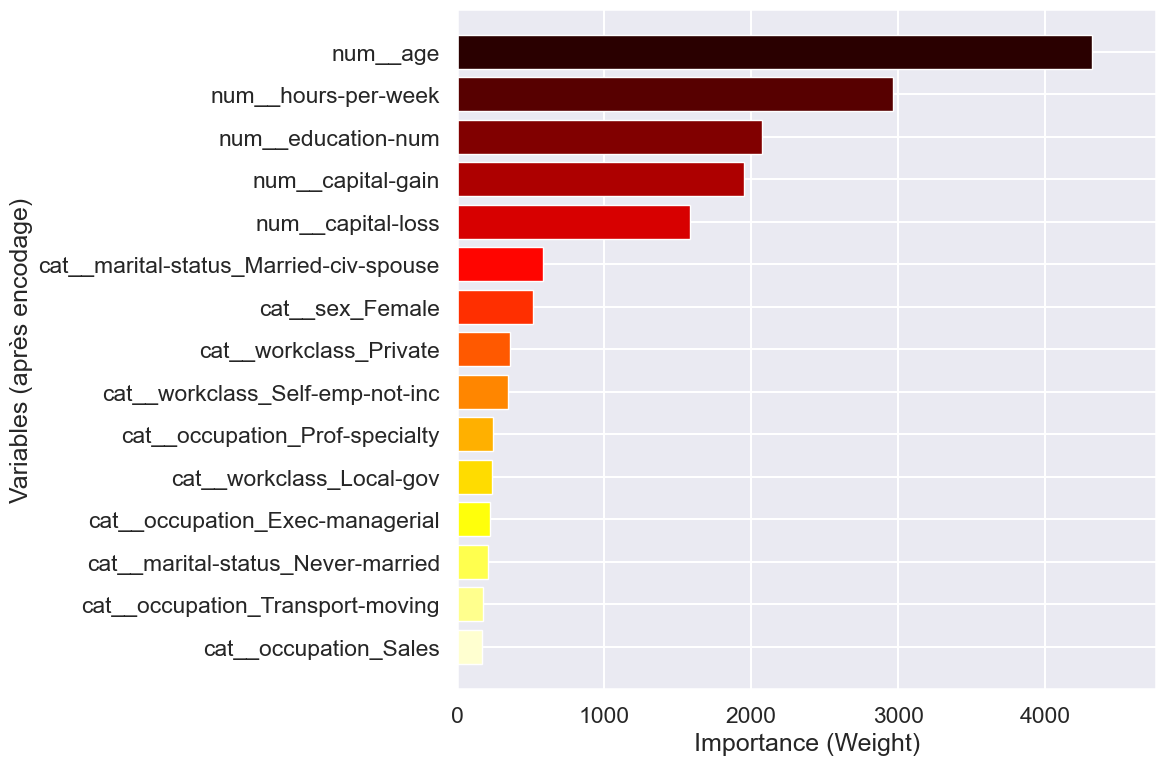
\includegraphics[width=\linewidth]{pictures/importance/feature_importance_weight.png}
		\caption{Variables les plus utilisées (Weight).}
    \end{subfigure}
    }
\end{figure}
\end{frame}

% --- SLIDE 9 : INTERPRÉTABILITÉ (LOCAL) ---
\begin{frame}{Déploiement et interprétabilité locale (SHAP)}
Le \mytexttt{Pipeline} final est sauvegardé via \mytexttt{joblib} pour simuler une inférence en production.\pause~Pour interpréter les résultats de la boîte noire, intégration des \textbf{SHapley Additive exPlanations} (SHAP).
    \pause
    \vspace{0.1cm}
    \begin{figure}[htb]
	\centering
	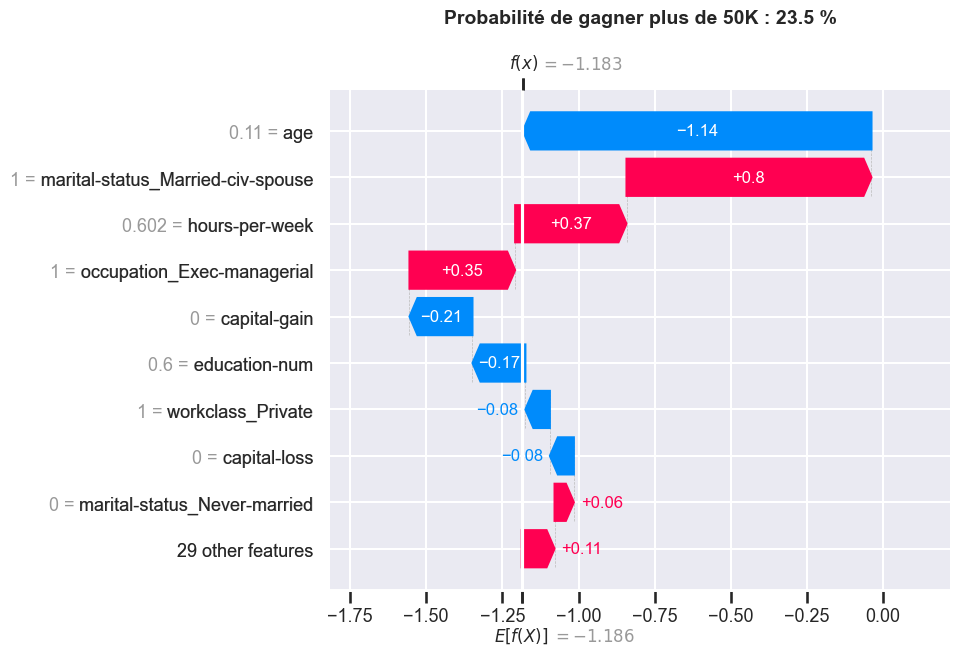
\includegraphics[width=0.5\textwidth]{pictures/inference/SHAP.png}
	\caption{Quelles caractéristiques ont joué dans la prédiction pour cet individu et comment ?}
	\end{figure}
\end{frame}

% --- SLIDE 10 : CONCLUSION ---
\begin{frame}{Conclusion}
    \textbf{Bilan du projet :}
    \pause
    \begin{itemize}
    		\item \textbf{Processus :} proche du \textbf{Cross-Industry Standard Process for Data Mining} (CRISP-DM).
    		\pause
        \item \textbf{Technique :} pipeline Scikit-Learn robuste, et des résultats reproductibles.
        \pause
        \item \textbf{Performance :} optimisation ciblée (F1-score) qui corrige les faiblesses du premier modèle (2021).
        \pause
        \item \textbf{Métier :} modèle auditable grâce à SHAP.
    		\pause
        \item \textbf{Perspectives :} tester d'autres modèles (autres ensemblistes, MLP, modèles de fondation tabulaires), interface graphique pour la production.
    \end{itemize}

    \vspace{0.5cm}
    \begin{center}
        \Large{\textbf{Merci pour votre attention !}}
    \end{center}
\end{frame}

\end{document}